\chapter{Concept of the algorithm}
\label{chap:algorithm}

In the following sections we are going to develop a mathematical and algorithmic framework that allows us to compute the GIT fan for the case of a torus acting on an affine variety. The concepts presented in this chapter base on \cite{gitfan_symmetry, gitfan}.

First, we describe the formal setup and introduce the notation being used in the upcoming chapters. In the second section we present an algorithm that is capable of identifying orbit cones. They play an important role in the theory since all GIT cones emerge from their intersections. Afterwards, we transform the problem of computing the GIT fan into the problem of traversing a graph and present a suitable algorithm. Third, we modify the previous algorithms such that symmetries of the affine variety may be exploited in order to reduce the problem size by a factor that relates to the size of the symmetry group. Finally, we give an counterexample that -- contrary to \cite{gitfan_symmetry} -- one cannot drop non-minimal orbit cones with respect to inclusion. For this reason, we leave out the minimisation process.

\section{The setup}
\label{section:setup}

Let $\field$ be an algebraically closed field of characteristic zero. We consider an algebraic group action of a $k$-dimensional torus $T$ on an affine variety $X$. Due to construction~\ref{construction:algebraic_torus}, we describe this setup by a set of integral vectors $q_i\in\integer^k$, $1\leq i \leq r$, and a suitable embedding of $X$ in $\field^r$ such that its vanishing ideal $\ideal \defeq I(X)$ is homogeneous w.r.t.
$$\deg(x_i) = q_i,\quad 1\leq i \leq r.$$
The vectors $q_i$ form the columns of a matrix $Q\in\field^{k\times r}$. By restricting $T$ to a lower dimensional subtorus if necessary, we may assume that $Q$ has rank $k$ without changing the orbits in $X$. Furthermore, we assume that $\ideal$ contains no monomials. As we will see later on, this assumption is equivalent to $X\cap (\field^*)^r \neq \emptyset$. On that account and the irreducibility of $X$, $X$ is located in at least one of the hyperplanes $\{x_i = 0\}$, $1\leq i \leq r$, iff the assumption does not hold. By ``forgetting" all variables with $X\cap \{x_i = 0\} = X$, we obtain an embedding of $X$ such that $X\cap (\field^*)^{r'} \neq \emptyset$ holds.

\section{Computing orbit cones}

In this section we describe orbit cones by faces of the positive orthant $\rational_{\geq 0}^r$, which we denote by $\gamma$.
\index{gamma@$\gamma$}%
From a combinatorial point of view these faces are subsets of $\{1,\dots,r\}$ such that whenever $e_i$ is a ray of a face, $i$ is located in the corresponding subset. A face $\gamma_0 \preceq \gamma$ defines a restriction $z_{\gamma_0}$ of any $r$\=/tuple of objects $z=(z_1,\dots,z_r)$ by setting
$$(z_{\gamma_0})_i =
\begin{cases}
z_i, & e_i\in\gamma_0 \\
0, & \text{else}
\end{cases}\quad 1\leq i \leq r.$$
We write $\ideal_{\gamma_0}$ for the ideal in $\field[\mathbf{x}_{\gamma_0}]$ that is obtained by sending all $x_i$ in $\ideal$ with $x_i\notin\gamma_0$ to zero.
\index{agamma0@$\ideal_{\gamma_0}$}%
Additionally, we define
$$\T_{\gamma_0} \defeq (\field^*)^r \cdot (1,\dots,1)_{\gamma_0},$$
which is the torus corresponding to $\gamma_0$.
\index{Tgamma0@$\T_{\gamma_0}$}%

\begin{defi}[\aface]
	A face $\gamma_0\preceq\gamma$ is called \emph{\aface{}} iff $X\cap \T_{\gamma_0} \neq \emptyset$.
	\index{aface@\aface}%
\end{defi}

\begin{prop}
	\label{prop:aface_orbit_cone_correspondence}
	The set
	$$\Omega_\ideal \defeq \left\{Q(\gamma_0)\ |\ \gamma_0\preceq\gamma \text{ is an } \ideal\text{\=/face}\right\}$$
	equals the collection of orbit cones as in Definition~\ref{defi:orbit_cone}.
	\index{Oa@$\Omega_\ideal$}%
\end{prop}
\begin{proof}
	Let $x\in X$. Set $I_x = \{1 \leq i \leq r\ |\ x_i \neq 0\}$ and $J_x = \{1 \leq i \leq r\ |\ x_i = 0\}$. We claim that
	$$S_T(x) = \langle q_i\ |\ i\in I_x\rangle.$$
	
	Let $i\in I_x$. Since $x_i\in\field[\mathbf{x}]$ does not send $x$ to zero, we have
	$$q_i = \deg(x_i)\in S_T(x).$$
	Now let $w\in S_T(x)$. Then there exists $f\in\field[\mathbf{x}]_w$ such that $f(x) \neq 0$. In particular, at least one monomial $\mathbf{x}^\alpha$ of $f$ does not send $x$ to zero, thus $\alpha_j = 0$ for all $j\in J_x$. On that account we have
	$$w = \deg(x^\alpha) = \sum_{i=1}^r \alpha_i q_i = \sum_{i\in I_x} \alpha_i q_i,$$
	proving the claim.
	
	If $\gamma_0\preceq\gamma$ is an \aface{}, we find a point $x\in X\cap \T_{\gamma_0}$. By the previous claim, its orbit monoid is generated by the columns $q_i$ of $Q$ with $e_i\in\gamma_0$. Consequently, $Q(\gamma_0)$ is the orbit cone of $x$ generated by $S_T(x)$.
	
	Conversely, consider the orbit cone of an arbitrary point $x\in X$. Let $\gamma_x$ be the face of $\gamma$ that is generated by the rays $e_i$ with $i\in I_x$. Then $\gamma_x$ is an \aface{}, since $x\in X\cap \T_{\gamma_x}$. With the same arguments as before, it follows that $Q(\gamma_x)$ is the orbit cone of $x$.
\end{proof}

The previous proposition shows that all orbit cones arise from \afaces{} and that every \aface{} yields an orbit cone. Thus, if we are able to develop computable criteria in order to implement a test for the \aface{} property, we can derive all orbit cones by applying $Q$. The next proposition provides us with a suitable criterion.

\begin{prop}
	\label{prop:aface_equivalence}
	Let $\gamma_0\preceq\gamma$ be a face and $I= \{1\leq i\leq r\ |\ e_i\in\gamma_0\}$. Then the following conditions are equivalent:
	\begin{enumerate}[label={\upshape(\roman*)}]
		\item $\gamma_0$ is an \aface{}, that is $X\cap \T_{\gamma_0} \neq \emptyset$,
		\label{enum_item:aface_equivalence_aface}
		\item $\ideal_{\gamma_0}$ does not contain a monomial,
		\label{enum_item:aface_equivalence_monomial}
		\item $(\ideal_{\gamma_0} : (\prod_{i\in I} x_i)^\infty) = \field[\mathbf{x}_{\gamma_0}]$.
		\label{enum_item:aface_equivalence_saturation}
	\end{enumerate}
\end{prop}
\begin{proof}
	\ref{enum_item:aface_equivalence_monomial} $\Leftrightarrow$ \ref{enum_item:aface_equivalence_saturation} immediately follows from the definition of saturated ideals (see Appendix~\ref{appendix:ideal_quotients}), which unravels to
	$$\left(\ideal_{\gamma_0} : \left(\prod_{i\in I} x_i\right)^\infty\right) = \left\{r\in \field[\mathbf{x}]\ \middle|\ \exists j\in\natural: r\cdot \left(\prod_{i\in I} x_i\right)^j \in \ideal_{\gamma_0}\right\}.$$
	If $\ideal_{\gamma_0}$ contains a monomial $x^\alpha$, we have that $(\prod_{i\in I} x_i)^j\in\ideal_{\gamma_0}$, where $j$ is the largest integer occurring in $\alpha$. Thus, $1\in (\ideal_{\gamma_0} : (\prod_{i\in I} x_i)^\infty)$ and therefore \ref{enum_item:aface_equivalence_saturation} follows. Otherwise, if \ref{enum_item:aface_equivalence_saturation} holds, a power of $\prod_{i\in I} x_i$, which is a monomial, is contained in $\ideal_{\gamma_0}$.
	
	\ref{enum_item:aface_equivalence_aface} $\Rightarrow$ 
	\ref{enum_item:aface_equivalence_monomial}: Choose a point $x\in X\cap \T_{\gamma_0}$. Assume that \ref{enum_item:aface_equivalence_monomial} does not hold, i.e. $\ideal_{\gamma_0}$ contains a monomial $\mathbf{x}^\alpha$, $\alpha = (\alpha_i)_{i\in I}$, that is obtained by sending all $x_i$, $i\notin I$, in a suitable $f\in\ideal$ to zero.
	Since $x\in\T_{\gamma_0}$, it holds that
	$$f(x) = \prod_{i\in I} x_i^{\alpha_i} \neq 0,$$
	contradicting $x\in X = V(\ideal)$.
	
	\ref{enum_item:aface_equivalence_monomial} $\Rightarrow$ 
	\ref{enum_item:aface_equivalence_aface}: Assume that $V(\ideal_{\gamma_0}) \subseteq V(\prod_{i\in I} x_i)$ holds. Then Hilbert's Nullstellensatz yields $j\in\natural$ such that $(\prod_{i\in I} x_i)^j\in\ideal_{\gamma_0}$, contradicting \ref{enum_item:aface_equivalence_monomial}. Hence, $V(\ideal_{\gamma_0}) \not\subseteq V(\prod_{i\in I} x_i)$. In particular, we find a point $z = (z_i)_{i\in I} \subseteq \field^*$ with $z\in V(\ideal_{\gamma_0})$. We extend $z$ to a point $\tilde{z}\in\T_{\gamma_0}$ by setting
	$$\tilde{z}_i = \begin{cases}
	z_i, & i\in I \\
	0, & \text{else}
	\end{cases}\quad 1\leq i \leq r.$$
	
	Let $f\in\ideal$ and $f_{\gamma_0}\in\ideal_{\gamma_0}$ be the reduction of $f$ by sending all variables $x_i$, $i\notin I$, to zero. Then we have
	$$f(\tilde{z}) = f_{\gamma_0}(z) = 0,$$
	since $z\in V(\ideal_{\gamma_0})$. We conclude that $\tilde{z}\in X$, showing \ref{enum_item:aface_equivalence_aface}.
\end{proof}

Next, we implement an algorithm computing $(I : (z_1\cdots z_n)^\infty)$ for arbitrary ideals $I\in\field[z_1,\dots,z_n]$. The algorithm presented here originates from \cite{gitfan_symmetry} and has been implemented in \gitfanlib. It relies on the following proposition that allows us to compute $(I : (z_i)^\infty)$ with relative ease by a small modification to the Buchberger's algorithm.

\begin{prop}[\phantom{}{\cite[Proposition 3.1]{gitfan_symmetry}}]
	\label{proposition:saturated_monomial}
	Let $\;>$ be a monomial ordering on $\field[\mathbf{z}]$ and $\mathcal{G}$ be a standard basis of $I$ with respect to $\;>$. Let $m\in\{1,\dots,n\}$. If $\;>$ satisfies
	\begin{equation}
		\label{equation:saturated_monomial_assumption}
		z_m \mid f\ \Leftrightarrow\ z_m \mid \text{LM}_>(f),
	\end{equation}
	then
	$$\left\{g\in\field[\mathbf{z}]\ \middle|\ z_m \centernot\mid g\ \mathrm{and}\ \exists i\in\natural_0: (z_m)^i \cdot g \in \mathcal{G}\right\}$$
	is a standard basis for the saturated ideal $I : (z_m)^\infty$. 
\end{prop}

\begin{remark}
	\label{remark:satisying_assumption_saturated_monomial}
	The negative reverse lexicographical ordering
	$$z^\alpha >_\text{rs} z^\beta\ \defequiv\ \exists i\in\{1,\dots,n\}: \alpha_i < \beta_i\ \text{and}\ \alpha_j = \beta_j\ \forall j\in\{i+1,\dots,n\}$$
	ensures that (\ref{equation:saturated_monomial_assumption}) is satisfied for $m=n$. Every monomial $z^\beta$ with $z_n \mid z^\beta$ is strictly smaller than any monomial $z^\alpha$ with $z_n \centernot\mid z^\alpha$, since $\alpha_n = 0 < \beta_n$. Note that (\ref{equation:saturated_monomial_assumption}) may hold for other values of $m$ by using a negative reverse lexicographical ordering after reordering the variables $z_1,\dots,z_n$.
	
	Unfortunately, $\;>_\text{rs}$ is no global ordering. However, if $I$ permits a weight vector $w\in\integer^n_{>0}$ such that $I$ is homogeneous, we consider the $w$\=/weighted degree ordering with tie-breaker $\;>_\text{rs}$, that is $(>_w, >_\text{rs})$. This ordering is global and satisfies (\ref{equation:saturated_monomial_assumption}) on $w$\=/homogeneous generators of $I$.
\end{remark}

Since we have
$$(I:(z_1\cdots z_n)^\infty) = (\dots((I:(z_1)^\infty):(z_2)^\infty):\dots : (z_n)^\infty)\quad\text{(see Appendix \ref{appendix:ideal_quotients})},$$
Proposition~\ref{proposition:saturated_monomial} allows us to compute $(I : (z_1\cdots z_n)^\infty)$ by alternating Mora's algorithm with $>_\text{rs}$ and the elimination of factors $z_i$. If a global ordering as in Remark~\ref{remark:satisying_assumption_saturated_monomial} is available, one can integrate the elimination process into the Buchberger's algorithm in order to speed up convergence. Algorithm~\ref{algo:saturated_monomial} (see also \cite[Algorithm 3.3]{gitfan_symmetry}) contains the necessary modifications.

\begin{algorithm}
	\caption{Computing the saturation at the product of all variables}
	\label{algo:saturated_monomial}
	
	\KwIn{A vector $w\in\integer^n_{>0}$ and a set $\mathcal{G}$ of $w$-homogenous polynomials such that $\langle \mathcal{G}\rangle = I$}
	\KwOut{A Gröbner basis for the saturation $(I:(z_1\cdots z_n)^\infty)$ with respect to the ordering $(>_w, >_\text{rs})$}
	\BlankLine
	$\mathcal{G} \leftarrow \{g / z^\alpha\ |\ g\in \mathcal{G}\ \text{and}\ \alpha\ \text{maximal such that}\ z^\alpha \mid g\}$\;
	\label{algo_line:saturated_monomial_preprocess_G}
	\For{$m=1,\dots,n$}{
		Let $\;>_m$ be $(>_w, >_\text{rs})$ where $\;>_\text{rs}$ is the negative reverse lexicographical ordering after reordering variables such that
		$$z_1 >_\text{rs} \dots >_\text{rs} z_{m-1} >_\text{rs} z_{m+1} >_\text{rs} \dots >_\text{rs} z_n >_\text{rs} z_m.$$
		
		\Repeat{$\mathcal{G} = \mathcal{H}$\label{algo_line:saturated_monomial_repeat_condition}}{
			$\mathcal{H} \leftarrow \mathcal{G}$\;
			\For{$f,g\in\mathcal{H}$}{
				$r \leftarrow \text{NF}_{>_m} (\text{spoly}_{>_m}(f,g),\mathcal{H})$\;
				\If{$r \neq 0$}{
					$r \leftarrow r / z^\alpha,\ \text{where}\ \alpha\ \text{is maximal such that}\ z^\alpha \mid g$\;
					$\mathcal{G} \leftarrow \mathcal{G} \cup \{r\}$\;
				}
			}
		}
	}
	\Return $\mathcal{G}$\;
\end{algorithm}

\begin{prop}
	Algorithm~\ref{algo:saturated_monomial} computes the saturation $(I:(z_1\cdots z_n)^\infty)$ as specified in pseudo code.
\end{prop}
\begin{proof}
	Similarly to the Buchberger's algorithm, whenever a new element $r$ is introduced to $\mathcal{G}$, its lead monomial $\text{LM}(r)$ is not contained in the lead ideal of $\langle \mathcal{G} \rangle$. Consequently, $\langle \mathcal{G} \rangle$ strictly increases. Since $\field[\mathbf{z}]$ is noetherian, eventually $\langle \mathcal{G} \rangle$ becomes stationary, implying that no new elements $r$ have been inserted. Hence, the condition in Line~\ref{algo_line:saturated_monomial_repeat_condition} holds eventually and the algorithm terminates.
	
	Denote by $\mathcal{G}_0$ the set $\mathcal{G}$ after executing Line~\ref{algo_line:saturated_monomial_preprocess_G} and by $\mathcal{G}_m$ the Gröbner basis after the $m$-iteration of the outmost loop. Set $I_m = \langle \mathcal{G}_m \rangle$.
	
	First, note that the elements inserted into $\mathcal{G}$ are contained in $(I:(z_1\cdots z_n)^\infty)$ and are not divisible by any monomials. Furthermore, they are $w$-homogeneous since NF and spoly preseve homogeneity. Consequently, $\mathcal{G}_m$ satisfies the assumption of Proposition~\ref{proposition:saturated_monomial} with respect to the ordering $\;>_m$. As no element of $\mathcal{G}_m$ is divisible by any monomial, it follows that $\mathcal{G}_m$ is saturated with respect to $z_m$. In particular, $(I_{m-1} : (z_m)^\infty) \subseteq I_m$. Appendix~\ref{appendix:ideal_quotients} states that saturations preserve inclusion, so that $I\subseteq I_0$ together with $(I_{m-1} : (z_m)^\infty) \subseteq I_m$ implies that
	$$(I:(z_1\cdots z_n)^\infty) = (\dots((I:(z_1)^\infty):(z_2)^\infty):\dots : (z_n)^\infty) \subseteq I_n$$
	by a simple induction. It follows that $\langle \mathcal{G}_m \rangle = I_m = (I:(z_1\cdots z_n)^\infty)$.
\end{proof}

Now we are able to compute all orbit cones $\Omega_\ideal^{(k)}$ of full dimension $k$ by Algorithm~\ref{algo:compute_orbit_cones}. Its correctness is a straightforward conclusion from  Proposition~\ref{prop:aface_orbit_cone_correspondence} and~\ref{prop:aface_equivalence}.

\begin{notation}
	Let $\mathcal{C}$ be a set of convex cones. Then we write $\mathcal{C}^{(k)}$ for the subset of all $k$\=/dimensional cones in $\mathcal{C}$.
	\index{C(k)@$\mathcal{C}^{(k)}$}%
\end{notation}

\begin{algorithm}
	\caption{Computing all full dimensional orbit cones}
	\label{algo:compute_orbit_cones}
	
	\KwIn{$\ideal$, $Q$}
	\KwOut{All orbit cones of $\Omega_\ideal^{(k)}$ dimension $k$}
	\BlankLine
	$\Omega \leftarrow \emptyset$\;
	\For{$\gamma_0\preceq \gamma$ with $\dim(Q(\gamma_0)) = k$}{
		$I \leftarrow \ideal_{\gamma_0}$\;
		$I_\text{sat} \leftarrow (I:(\prod_{e_i\in\gamma_0} x_i)^\infty)$%
			\Comment*[r]{by Algorithm~\ref{algo:saturated_monomial}}
		\If{$I_\text{sat} = \field[\mathbf{x}_{\gamma_0}]$}{
			$\Omega \leftarrow \Omega \cup \{Q(\gamma_0)\}$\;
		}
	}
	\Return $\Omega$\;
\end{algorithm}

\section{Traversing the GIT fan}

With the full dimensional orbit cones at hand, we are able to determine the GIT fan $\Sigma_T(X)$ defined by the torus action $T$ on the variety $X$. Since the support of $\Sigma_T(X)$ is the image $Q(\gamma)$ and $Q$ has rank $k$, it follows that $\Sigma_T(X)$ is a $k$-dimensional quasifan with convex support.
By Lemma~\ref{lemma:convex_fan_maximal_cones}, it suffices to consider only the full dimensional GIT cones in $\Sigma_T(X)^{(k)}$. These yield a graph structure by relating two GIT cones sharing a common facet.

\begin{defi}
	The graph $\mathcal{G}(\Sigma_T(X))$ of the GIT fan $\Sigma_T(X)$ is the undirected graph with nodes in $\Sigma_T(X)^{(k)}$ and the symmetric relation
	$$E_{\mathcal{G}(\Sigma_T(X))} \defeq \left\{\{\lambda, \mu\} \mid \lambda, \mu \in \Sigma_T(X)^{(k)} \text{ and }\lambda \cap \mu \text{ is a facet of both }\lambda\text{ and }\mu\right\}.$$
	\index{GSigmaTX@$\mathcal{G}(\Sigma_T(X))$}%
	\index{EGSigmaTX@$E_{\mathcal{G}(\Sigma_T(X))}$}%
\end{defi}

\begin{prop}
	\label{proposition:git_fan_connected}
	The graph $\mathcal{G}(\Sigma_T(X))$ is connected.
\end{prop}
\begin{proof}
	Let $\lambda_s, \lambda_t\in\Sigma_T(X)^{(k)}$ and choose a point $x_s\in\lambda_s^\circ$. Let $S$ be the set of points that are not located on a line through $x_s$ and a point of a face of dimension $k-2$ or lower, that is
	$$S = \left\{p\in|\Sigma|\ \middle|\ \overline{x_s p} \cap \left(\bigcup_{\lambda\in\Sigma_T(X)^{(\leq k-2)}} \lambda\right) = \emptyset\right\}.$$
	Obviously, for every point $p\in |\Sigma|\setminus S$ we can choose $\lambda\in\Sigma_T(X)^{(\leq k-2)}$ such that $p$ is located in the subspace generated by $x_s$ and $\lambda$. As the dimension of this subspace is at most $k-1$, we conclude that the complement of $S$ in $|\Sigma|$ is contained in a finite union of hyperplanes.
	For dimensional reasons, any non\=/empty open set $U$ in $|\Sigma|$ with respect to the euclidean topology satisfies
	$$U\cap S \neq \emptyset.$$
	This shows that there exists a point $x_t\in\lambda_t^\circ$ such that $x_t\in S$.
	
	Consider the connecting line $\ell \defeq \overline{x_s x_t}$. We have $\ell\subseteq|\Sigma_T(X)|$, because $|\Sigma_T(X)|$ is convex. By the definition of $S$, $\ell$ only contains points in the relative interior of $(k-1)$- or $k$\=/dimensional cones. Furthermore, $\ell$ intersects every $(k-1)$\=/dimensional cone $\lambda$ in at most one point. Otherwise, $\ell$ would be contained in the hyperplane spanned by $\lambda$ due to Bézout's theorem. Then, $\ell$ also would intersect a proper face of $\lambda$ with dimension lower than $k-1$, contradicting $x_t\in S$.
	
	Since the relative interior of a $k$\=/dimensional cone is open and convex, its intersection with $\ell$ is an open interval in $\ell$. We conclude that $\ell$ has the form
	
	\begin{center}
		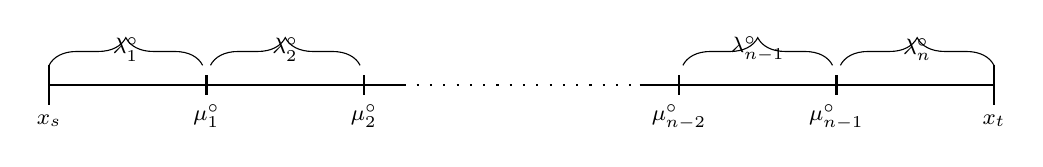
\begin{tikzpicture}
		\draw[thick] (0,0) -- (4.5,0);
		\draw[thick,loosely dotted] (4.5,0) -- (7.5,0);
		\draw[thick] (7.5,0) -- (12,0);
		\draw[thick] (0,-0.25) -- (0,0.25);
		\draw[thick] (12,-0.25) -- (12,0.25);
		\draw[thick] (2,-0.125) -- (2,0.125);
		\draw[thick] (4,-0.125) -- (4,0.125);
		\draw[thick] (8,-0.125) -- (8,0.125);
		\draw[thick] (10,-0.125) -- (10,0.125);
		
		\draw[decorate,decoration={brace,amplitude=10pt}]
			(0,0.25) -- (1.95,0.25) node [midway, yshift=0.2cm] {\footnotesize $\lambda_1^\circ$};
			\draw[decorate,decoration={brace,amplitude=10pt}]
			(2.05,0.25) -- (3.95,0.25) node [midway, yshift=0.2cm] {\footnotesize $\lambda_2^\circ$};
			\draw[decorate,decoration={brace,amplitude=10pt}]
			(8.05,0.25) -- (9.95,0.25) node [midway, yshift=0.2cm] {\footnotesize $\lambda_{n-1}^\circ$};
			\draw[decorate,decoration={brace,amplitude=10pt}]
			(10.05,0.25) -- (12,0.25) node [midway, yshift=0.2cm] {\footnotesize $\lambda_n^\circ$};
		\node[anchor=north] at (0,-0.25) {\footnotesize $x_s$};
		\node[anchor=north] at (2,-0.125) {\footnotesize $\mu_1^\circ$};
		\node[anchor=north] at (4,-0.125) {\footnotesize $\mu_2^\circ$};
		\node[anchor=north] at (8,-0.125) {\footnotesize $\mu_{n-2}^\circ$};
		\node[anchor=north] at (10,-0.125) {\footnotesize $\mu_{n-1}^\circ$};
		\node[anchor=north] at (12,-0.25) {\footnotesize $x_t$};
		\end{tikzpicture}
	\end{center}
	
	with $\lambda_i\in\Sigma_T(X)^{(k)}$ for all $1\leq i \leq n$ and $\mu_j\in\Sigma_T(X)^{(k-1)}$ for all $1\leq j \leq n-1$. In particular, the point in $\mu_j^\circ\cap \ell$ is contained in $\lambda_j$ and $\lambda_{j+1}$, so that $\mu_j$ is a facet of $\lambda_j$ and $\lambda_{j+1}$. For this reason, $\lambda_1,\lambda_2,\dots,\lambda_n$ constitutes a path in $\mathcal{G}(\Sigma_T(X))$ from $\lambda_1$ to $\lambda_n$. Since $x_s\in\lambda_1$ and $x_t\in\lambda_n$, it follows that $\lambda_1 = \lambda_s$ and $\lambda_n = \lambda_t$.
\end{proof}

Proposition~\ref{proposition:git_fan_connected} allows us to determine all full dimensional GIT cones by traversing the graph $\mathcal{G}(\Sigma_T(X))$. For this reason we require a routine for computing all GIT cones related to a given GIT cone. We begin with some elementary observations about GIT cones that also become important when encoding GIT cones in section~\ref{sec:git_cone_management}.

\begin{notation}
	Let $p\in Q(\gamma)$. Then $\lambda(p)$ denotes the associated GIT cone with respect to the torus action of $T$ on $X$, that is
	$$\lambda(p) \defeq \bigcap_{p\in\sigma\in\Omega_\ideal} \sigma$$
	due to Propositon~\ref{prop:aface_orbit_cone_correspondence}.
	\index{lambdap@$\lambda(p)$}%
\end{notation}

\begin{lemma}
	\label{lemma:git_cones_elementary_properties}
	Let $p\in Q(\gamma)$ such that $\lambda \defeq \lambda(p)\in\Sigma_T(X)^{(k)}$. Then we have
	\begin{enumerate}[label={\upshape(\roman*)}]
		\item $\lambda = \bigcap\limits_{p\in\sigma\in\Omega_\ideal^{(k)}}\sigma,$
			\label{enum_item:git_cones_full_dim_orbit_cones}
		\item $p\in\sigma\ \Leftrightarrow\ \lambda\subseteq\sigma\quad\forall\sigma\in\Omega_\ideal^{(k)},$
			\label{enum_item:git_cones_defining_orbit_cones}
		\item $\lambda = \bigcap\limits_{\lambda\subseteq\sigma\in\Omega_\ideal^{(k)}}\sigma,$
			\label{enum_item:git_cones_enclosed_orbit_cones}
		\item $\lambda = \lambda(q)\quad \forall q\in\lambda^\circ.$
			\label{enum_item:git_cones_relative_interior}
	\end{enumerate}
\end{lemma}
\begin{proof}
	\ref{enum_item:git_cones_full_dim_orbit_cones} is trivial since dimensions do not increase when intersecting. \ref{enum_item:git_cones_defining_orbit_cones} clearly holds by the definition of $\lambda$. \ref{enum_item:git_cones_enclosed_orbit_cones} is an immediate consequence of \ref{enum_item:git_cones_full_dim_orbit_cones} and \ref{enum_item:git_cones_defining_orbit_cones}.
	
	Let $q\in\lambda^\circ$. Since $q$ is contained in all $\sigma\in\Omega_\ideal^{(k)}$ such that $p\in\sigma$, it follows that $\lambda(q)\subseteq\lambda$. If the inequality would be proper, $\lambda(q)$ would be a proper face of $\lambda$ containing $q$, contradicting $q\in\lambda^\circ$.
\end{proof}

\begin{algorithm}
	\caption{Computing all related GIT cones}
	\label{algo:compute_git_cone_neighbours}
	
	\KwIn{A full dimensional GIT cone $\lambda\in\Sigma_T(X)^{(k)}$}
	\KwOut{All full dimensional GIT cones $\mu\in\Sigma_T(X)^{(k)}$ such that $\lambda\cap\mu$ is a common facet of $\lambda$ and $\mu$}
	\BlankLine
	$\mathcal{N} \leftarrow \emptyset$\;
	\For{$\vartheta\preceq \lambda$ being a facet of $\lambda$ with $\vartheta^\circ\cap\partial Q(\gamma) = \emptyset$}{
		Let $n$ be an inner-pointing normal of $\vartheta$\;
		Choose $v\in\vartheta^\circ$\;
		Choose small $\varepsilon > 0$\;
		$q \leftarrow v - \varepsilon n$\;
		\While{$v\notin\lambda(q)$ \label{algo_line:compute_git_cone_neighbours_while}}{
			$\varepsilon \leftarrow \varepsilon / 2$\;
			$q \leftarrow v - \varepsilon n$\;
		}
		$\mathcal{N} \leftarrow \mathcal{N} \cup \{\lambda(q)\}$\;
	}
	\Return $\mathcal{N}$\;
\end{algorithm}

\begin{prop}
	Algorithm~\ref{algo:compute_git_cone_neighbours} computes all neighbours for a given node in $\mathcal{G}(\Sigma_T(X))$.
\end{prop}

\begin{proof}
	First, note that for $\tau\in\Sigma_T(X)^{(k-1)}$ with normal $n$ and relative inner point $v$ every $\sigma\in\Sigma_T(X)^{(k)}$ with $\tau\preceq\sigma$ has to contain either $v-\varepsilon n$ or $v+\varepsilon n$ in its relative interior for sufficiently small $\varepsilon$. For this reason there exist exactly two cones with this property iff $\tau^\circ\cap\partial Q(\gamma) = \emptyset$ and one cone otherwise. If two cones exist, they are separated by the hyperplane spanned by $\tau$, so that the intersection is $\tau$.
	
	We reuse the notations introduced in Algorithm~\ref{algo:compute_git_cone_neighbours}. Let $\vartheta$ be a facet of $\lambda$ with $\vartheta^\circ\cap\partial Q(\gamma) = \emptyset$.
	Let $v\in\vartheta^\circ$ and $n$ an inner\=/pointing normal of $\vartheta$. Because of $v\in Q(\gamma)^\circ$, there exists an $\varepsilon > 0$ such that the connecting line $\ell_\varepsilon \defeq \overline{v(v-\varepsilon n)}$ is contained in $Q(\gamma)$. Since cones are convex, all cones $\mu\in\Sigma_T(X)^{(<k)}$ intersect with $\ell_\varepsilon$ in a possibly empty interval $I_\mu$. If $v\in I_\mu$, it follows that $\vartheta = \mu$, since $v\in\vartheta^\circ$ and $\mu$ has at most dimension $k-1$. Due to $|\Sigma_T(X)^{(<k)}| < \infty$, we can choose $\varepsilon$ sufficiently small such that the only cone with dimension $<k$ intersecting $\ell_\varepsilon$ is given by $\vartheta$. By the definition of $n$, we have $\ell_\varepsilon \cap \vartheta = \{v\}$.
	
	It follows that the connected space $\ell_\varepsilon \setminus \{v\}$ is covered by disjoint open intervals $\ell_\varepsilon \cap \mu^\circ$, $\mu\in\Sigma_T(X)^{(k)}$, and thus we have $$\ell_\varepsilon \setminus \{v\} = \ell_\varepsilon \cap \mu_0^\circ$$
	for a suitable $\mu_0\in\Sigma_T(X)^{(k)}$. By Lemma~\ref{lemma:git_cones_elementary_properties}, it follows that $\mu_0 = \lambda(v-\varepsilon n)$. The closure $\mu_0$ of $\mu_0^\circ$ contains $v$. Hence, the loop in Line~\ref{algo_line:compute_git_cone_neighbours_while} terminates. In particular, $\vartheta\preceq\mu_0$ and $\mu_0$ is the unique cone unequal to $\lambda$ with this property.
\end{proof}

\begin{remark}
	Since cones are invariant with respect to scaling, one may assume $v,n\in\integer^k$ and consider $mv-n$ for sufficiently large $m\in\natural$ instead of $v-\varepsilon n$. Hence, Algorithm~\ref{algo:compute_git_cone_neighbours} may be realised by only integer operations.
\end{remark}

Finally, Algorithm~\ref{algo:compute_git_cones} describes a graph traversal and returns all full dimensional GIT cones by Proposition~\ref{proposition:git_fan_connected}.

\begin{algorithm}
	\caption{Computing all full dimensional GIT cones}
	\label{algo:compute_git_cones}
	
	\KwIn{$Q(\gamma),\ \Omega_\ideal^{(k)}$}
	\KwOut{$\Sigma_T(X)^{(k)}$}
	\BlankLine
	\Repeat{$\dim(\lambda(p)) = k$}{
		Choose random point $p\in Q(\gamma)$\;
	}
	$\mathcal{C} \leftarrow \{\lambda(p)\}$\;
	$\mathcal{F} \leftarrow \{\lambda(p)\}$\;
	\While{$\mathcal{F}\neq \emptyset$}{
		Choose $\lambda\in\mathcal{F}$\;
		$\mathcal{F} \leftarrow \mathcal{F} \setminus \{\lambda\}$\;
		\For(\Comment*[f]{by Algorithm~\ref{algo:compute_git_cone_neighbours}}){$\mu$ with $\{\lambda,\mu\}\in E_{\mathcal{G}(\Sigma_T(X))}$}{
			\If{$\mu\notin\mathcal{C}$}{
				$\mathcal{C} \leftarrow \mathcal{C} \cup \{\mu\}$\;
				$\mathcal{F} \leftarrow \mathcal{F} \cup \{\mu\}$\;
			}
		}
	}
	\Return $\mathcal{C}$\;
\end{algorithm}

\section{Exploiting symmetry}
\label{sec:exploiting_symmetry}

In this section we modify Algorithm~\ref{algo:compute_git_cones} such that symmetries of $T$ acting on $X$ are taken into account, reducing the size of the traversed graph without loosing information. On that account, we include a symmetry group $\mathcal{S}$ in our setup.

\begin{defi}[\phantom{}{\cite[Definition 4.1]{gitfan_symmetry}}]
	\label{definition:symmetry_group}
	A \emph{symmetry group} of the action of $T$ on $X$ is a subgroup $\mathcal{S}$ of the symmetric group $\mathcal{S}_r$ such that there are group actions
	\begin{alignat*}{5}
		\mathcal{S} \quad\times\quad & \field[\mathbf{x}] && \quad\rightarrow\quad \field[\mathbf{x}],\quad & (\sigma, x_i) & \quad\mapsto\quad \sigma x_i \defeq c_{\sigma,i} \cdot x_{\sigma(i)} \\
		\mathcal{S} \quad\times\quad & \rational^r && \quad\rightarrow\quad \rational^r,\quad & (\sigma, e_i) & \quad\mapsto\quad \sigma e_i \defeq e_{\sigma(i)}
	\end{alignat*}
	with $c_\sigma\in(\field^*)^r$ such that $\mathcal{S}\ideal = \ideal$ holds and
	$$\sigma \ker(Q) \subseteq \ker(Q)\quad\forall\sigma\in \mathcal{S}.$$
\end{defi}

\begin{remark}
	\label{remark:symmetry_group_on_image}
	Let $\sigma\in\mathcal{S}$. The condition $\sigma \ker(Q) \subseteq \ker(Q)$ allows us to construct $A_\sigma\in\text{GL}(k,\rational)$ such that
	\begin{center}
		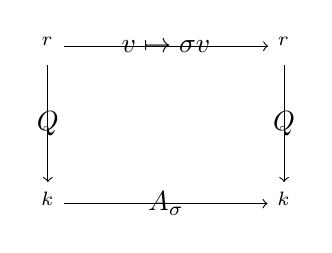
\begin{tikzpicture}
		\node (lt) {$\rational^r$};
		\node (rt) at (3,0) {$\rational^r$};
		\node (lb) at (0,-2) {$\rational^k$};
		\node (rb) at (3,-2) {$\rational^k$};
		\draw[->] (lt) to node {$v\mapsto \sigma v$} (rt);
		\draw[->] (lb) to node {$A_\sigma$} (rb);
		\draw[->] (lt) to node [swap] {$Q$} (lb);
		\draw[->] (rt) to node {$Q$} (rb);
		\end{tikzpicture}
	\end{center}
	commutes. Hence, the group action of $\mathcal{S}$ on $\rational^r$ induces a group action of $\mathcal{S}$ on $\rational^k$ with $(\sigma,v) \mapsto A_\sigma v$, such that the map defined by $Q$ becomes equivariant.
	
	We define $A_\sigma$ as follows: For $i\in\{1,\dots,k\}$, choose $v_i\in\rational^r$ such that $Q v_i = e_i\in\rational^k$. Then the $i$\=/th column of $A_\sigma$ is given by $Q(\sigma v_i)$. By construction, the diagram commutes on the subspace $T\subseteq\rational^r$ with basis $\{v_1,\dots,v_k\}$. It also commutes on $\ker(Q)$, sending all $v\in\ker(Q)$ to $0$ due to $\sigma v\in\ker(Q)$. We conclude that the diagram commutes on all $\rational^r = \ker(Q) \oplus T$.
	
	Since we have
	$$\Im(A_\sigma) = Q(\sigma\rational^r) = Q(\rational^r) = k,$$
	$A_\sigma$ is invertible.
\end{remark}

\begin{lemma}[\phantom{}{\cite[Lemma 4.7]{gitfan_symmetry}}]
	\label{lemma:symmetry_group_on_afaces}
	The action $\mathcal{S}\acts\rational^r$ induces an action of $\mathcal{S}$ on the set of \afaces{}.
\end{lemma}
\begin{proof}
	Let $\sigma\in\mathcal{S}$ and $\gamma_0\preceq\gamma$. We have to show that $\sigma\gamma_0$ is again an \aface{}. Since $\mathcal{S}$ permutes the canonical unit vectors, $\sigma\gamma_0$ is a face of $\gamma$. Let $x\in X\cap \T_{\gamma_0}$. We define $z\in\field^r$ such that
	$$z_i = c_{\sigma^{-1},i} \cdot x_{\sigma^{-1}(i)}\quad\forall 1\leq i \leq r$$
	with $c_{\sigma^{-1}}$ as in Definition~\ref{definition:symmetry_group}. It holds that
	$$
	e_i\in\sigma\gamma_0
	\ \Leftrightarrow\ e_{\sigma^{-1}(i)}\in\gamma_0
	\ \Leftrightarrow\ x_{\sigma^{-1}(i)} \neq 0
	\ \Leftrightarrow\ z_i = c_{\sigma^{-1},i} \cdot x_{\sigma^{-1}(i)} \neq 0
	\quad\forall 1\leq i\leq r,
	$$
	implying $z\in\T_{\sigma\gamma_0}$. Let $f\in\ideal$. By construction, we have $f(z) = (\sigma^{-1}f)(x)$. Now, $\sigma^{-1}f\in\ideal$ and $x$ vanishes on $\ideal$, so that $f(z) = 0$. For this reason $z\in X = V(\ideal)$ holds and $\sigma\gamma_0$ is an \aface{}.
\end{proof}

\begin{prop}
	\label{proposition:symmetry_group_on_orbit_cones}
	The action $\mathcal{S}\acts\rational^k$ introduced in Remark~\ref{remark:symmetry_group_on_image} induces an action $\mathcal{S}\acts\Omega_\ideal^{(k)}$. In particular, $\mathcal{S}$ acts on $\Sigma_T(X)^{(k)}$.
\end{prop}
\begin{proof}
	Let $\sigma\in\mathcal{S}$ and $Q(\gamma_0)\in\Omega_\ideal$ with $\gamma_0\preceq\gamma$ being an \aface{}. We show that $\sigma Q(\gamma_0)\in\Omega_\ideal^{(k)}$. By Remark~\ref{remark:symmetry_group_on_image}, $Q$ is equivariant. It follows that $\sigma Q(\gamma_0) = Q(\sigma\gamma_0)$. Since $\sigma\gamma_0$ is an \aface{} by Lemma~\ref{lemma:symmetry_group_on_afaces}, we have $\sigma Q(\gamma_0)\in\Omega_\ideal$.
	
	If $\lambda(p)$ is a GIT cone, then $\sigma \lambda(p)$ is the GIT cone associated to $A_\sigma p$, as it holds that
	$$A_\sigma p \in A_\sigma \vartheta = \sigma \vartheta \ \Leftrightarrow\ p\in \vartheta\quad \forall \vartheta\in\Omega_\ideal.$$
	Hence, $\mathcal{S}$ also acts on $\Sigma_T(X)$.
	
	Note that the action of $\mathcal{S}$ on cones in $\rational^k$ preserves dimensions because the matrices $A_\sigma$ are invertible. Consequently, we can restrict the actions on $\Omega_\ideal$ and $\Sigma_T(X)$ to cones of the fixed dimension $k$.
\end{proof}

Later on in chapter~\ref{chapter:moduli_space_of_pointed_stable_curves}, we are going to intersect the GIT fan with the cone of movable divisor classes of a Mori dream space. If this cone is invariant under the action of $\mathcal{S}$ on $\rational^k$, it suffices to intersect it with a representative system of orbit cone orbits only. The following proposition together with Remark~\ref{remark:cone_of_divisor_classes_in_mn_context} states the cone's invariance. 

\begin{prop}
	\label{prop:invariance_moving_cone}
	The convex cone
	$$\bigcap_{\gamma_0 \preceq \gamma\ \mathrm{facet}} Q(\gamma_0)\subseteq \rational^k$$
	is invariant with respect to the action $\mathcal{S}\acts \rational^k$.
\end{prop}
\begin{proof}
	Let $\sigma\in\mathcal{S}$. Since permutations in $\mathcal{S}_r$ permute the subsets of $\{1,\dots,r\}$ with cardinality $r-1$, the facets of $\gamma$ are permuted by $\sigma$. It follows that
	$$\sigma\cdot\left(\bigcap_{\gamma_0 \preceq \gamma\ \mathrm{facet}} Q(\gamma_0) \right)
	= \bigcap_{\gamma_0 \preceq \gamma\ \mathrm{facet}} \sigma\cdot Q(\gamma_0)
	= \bigcap_{\gamma_0 \preceq \gamma\ \mathrm{facet}} Q(\sigma \gamma_0)
	= \bigcap_{\gamma_0 \preceq \gamma\ \mathrm{facet}} Q(\gamma_0).$$
\end{proof}

Taking the symmetry group $\mathcal{S}$ into account, it suffices to traverse the following graph in order to determine the GIT fan.

\begin{defi}
	The graph $\mathcal{G}_\mathcal{S}(\Sigma_T(X))$ is the undirected graph with nodes in
	$$\faktor{\Sigma_T(X)^{(k)}}{\mathcal{S}}$$ 
	and the symmetric relation
	$$E_{\mathcal{G}_\mathcal{S}(\Sigma_T(X))} \defeq \left\{\{\mathcal{S}\lambda, \mathcal{S}\mu\}\ \middle|\ \{\lambda, \mu\} \in  E_{\mathcal{G}(\Sigma_T(X))}\right\}.$$
	\index{GSSigmaTX@$\mathcal{G}_\mathcal{S}(\Sigma_T(X))$}%
	\index{EGSSigmaTX@$E_{\mathcal{G}_\mathcal{S}(\Sigma_T(X))}$}%
\end{defi}

\begin{remark}
	Since $\mathcal{G}(\Sigma_T(X))$ is connected, it follows that the graph $\mathcal{G}_\mathcal{S}(\Sigma_T(X))$ is connected.
\end{remark}

\begin{algorithm}
	\caption{Computing all neighbours of a GIT cone orbit}
	\label{algo:git_cone_orbit_neighbours}
	
	\KwIn{A GIT cone orbit $\O\in\faktor{\Sigma_T(X)^{(k)}}{\mathcal{S}}$}
	\KwOut{All GIT cone orbits $\O_\mathcal{N}\in\faktor{\Sigma_T(X)^{(k)}}{\mathcal{S}}$ such that $\{\O, \O_\mathcal{N}\}\in E_{\mathcal{G}_\mathcal{S}(\Sigma_T(X))}$}
	\BlankLine
	$\mathcal{N} \leftarrow \emptyset$\;
	Choose $\lambda$ such that $\O = \mathcal{S}\lambda$\;
	\For(\Comment*[f]{by Algorithm~\ref{algo:compute_git_cone_neighbours}}){$\mu$ such that $\{\lambda,\mu\}\in E_{\mathcal{G}(\Sigma_T(X))}$\label{algo_line:git_cone_orbit_neighbours_loop}}{
		$\mathcal{N}\leftarrow \mathcal{N} \cup \{\mathcal{S}\mu\}$\;
	}
	\Return $\mathcal{N}$\;
\end{algorithm}

\begin{prop}
	Algorithm~\ref{algo:git_cone_orbit_neighbours} computes all neighbours of a node in $\mathcal{G}_\mathcal{S}(\Sigma_T(X))$.
\end{prop}
\begin{proof}
	We reuse the notation of Algorithm~\ref{algo:git_cone_orbit_neighbours}. Clearly, for all  $\O_\mathcal{N}\in\mathcal{N}$ it holds that $\{\O,\O_\mathcal{N}\}\in E_{\mathcal{G}_\mathcal{S}(\Sigma_T(X))}$.
	
	Conversely, let $\O_\mathcal{N}\in\Sigma_T(X)^{(k)}/\mathcal{S}$ such that $\{\O,\O_\mathcal{N}\}\in E_{\mathcal{G}_\mathcal{S}(\Sigma_T(X))}$. Then there exist $\lambda',\mu'\in\Sigma_T(X)^{(k)}$ such that $\{\lambda', \mu'\}\in E_{\mathcal{G}(\Sigma_T(X))}$ and $\O = \mathcal{S}\lambda'$, $\O_\mathcal{N} = \mathcal{S}\mu'$. Let $\sigma\in\mathcal{S}$ such that $\lambda' = \sigma\lambda$. Let $\vartheta$ be the common facet of $\lambda'$ and $\mu'$ and $n_{\lambda'}$, $n_{\mu'}$ the corresponding inner\=/pointing normals. Then $\sigma^{-1}\vartheta$ is the common facet of $\sigma^{-1}\lambda'$ and $\sigma^{-1}\mu'$ with inner\=/pointing normals $(A_{\sigma^{-1}}^*)^{-1} n_{\lambda'}$ and $(A_{\sigma^{-1}}^*)^{-1} n_{\mu'}$, where $A_{\sigma^{-1}}^*$ is the classical adjoint of $A_{\sigma^{-1}}$. In particular, $\{\lambda, \sigma^{-1}\mu'\}\in E_{\mathcal{G}(\Sigma_T(X))}$. Due to $\O = \mathcal{S}\lambda$ and $\O_\mathcal{N} = \mathcal{S}\mu' = \mathcal{S}(\sigma^{-1}\mu')$, it follows that $\O_\mathcal{N}$ is added to $\mathcal{N}$ when iterating the loop in Line~\ref{algo_line:git_cone_orbit_neighbours_loop}.
\end{proof}

Finally, Algorithm~\ref{algo:compute_git_cone_orbits} computes all full dimensional GIT cone orbits. It arises from Algorithm~\ref{algo:compute_git_cones} by small modifications coloured in red.

\begin{algorithm}
	\caption{Computing all full dimensional GIT cone orbits}
	\label{algo:compute_git_cone_orbits}
	
	\KwIn{$Q(\gamma),\ \Omega_\ideal^{(k)}$}
	\KwOut{$\textcolor{red}{\faktor{\textcolor{black}{\Sigma_T(X)^{(k)}}}{\mathcal{S}}}$}
	\BlankLine
	\Repeat{$\dim(\lambda(p)) = k$}{
		Choose random point $p\in Q(\gamma)$\;
	}
	$\mathcal{C} \leftarrow \{\textcolor{red}{\mathcal{S}}\lambda(p)\}$\;
	$\mathcal{F} \leftarrow \{\textcolor{red}{\mathcal{S}}\lambda(p)\}$\;
	\While{$\mathcal{F}\neq \emptyset$}{
		Choose $\textcolor{red}{\O}\in\mathcal{F}$\;
		$\mathcal{F} \leftarrow \mathcal{F} \setminus \{\textcolor{red}{\O}\}$\;
		\For(\Comment*[f]{by Algorithm~\textcolor{red}{\ref{algo:git_cone_orbit_neighbours}}}){$\textcolor{red}{\O_\mathcal{N}}$ with $\{\textcolor{red}{\O,\O_\mathcal{N}}\}\in E_{\mathcal{G}_{\textcolor{red}{\mathcal{S}}}(\Sigma_T(X))}$}{
			\If{$\textcolor{red}{\O_\mathcal{N}}\notin\mathcal{C}$}{
				$\mathcal{C} \leftarrow \mathcal{C} \cup \{\textcolor{red}{\O_\mathcal{N}}\}$\;
				$\mathcal{F} \leftarrow \mathcal{F} \cup \{\textcolor{red}{\O_\mathcal{N}}\}$\;
			}
		}
	}
	\Return $\mathcal{C}$\;
\end{algorithm}

\section{Counterexample: Removal of non-minimal orbit cones}

By discarding as many orbit cones as possible in $\Omega_\ideal^{(k)}$ without affecting the resultant GIT fan, one can speed up the computation of the associated GIT cone $\lambda(p)$ of an arbitrary point $p\in Q(\gamma)$. Clearly, one can discard all orbit cones being a union or intersection of the remaining ones. However, the approach in \cite{gitfan_symmetry} of removing all non\=/minimal cones in $\Omega_\ideal^{(k)}$ with respect to inclusion is flawed. Fortunately, \cite[Theorem 1.1]{gitfan_symmetry} still holds as all non-minimal orbit cones are unions of minimal ones for the \msix{} example.

Consider the following scenario. Let $f = x_1x_3+x_2x_4+x_5\in \field[x_1,x_2,x_3,x_4,x_5]$. Set  $\ideal := \langle x_3, x_4\rangle \cdot \langle f\rangle$ and
$$Q = (q_1, q_2, q_3, q_4, q_5) := \begin{pmatrix}
0 & 0 & 1 & 1 & 1 \\
1 & 0 & 0 & 1 & 1 \\
1 & 1 & 1 & 1 & 2 
\end{pmatrix}.$$

It is easy to see that the matrix $Q$ is of full rank 3 and that $f$ and thus $\ideal$ are homogeneous with respect to the $\integer^3$\=/grading induced by $Q$. Furthermore, $\ideal$ does not contain any monomials. Overall, $\ideal$ and $Q$ constitute a valid setup in the sense of section~\ref{section:setup}. The $\ideal$-faces with full dimensional image in $Q(\gamma)$ are given by
\begin{align*}
\gamma_1 &:=\langle e_1, e_2, e_5\rangle \\
\gamma_2 &:=\langle e_1, e_2, e_3, e_5\rangle \\
\gamma_3 &:=\langle e_1, e_2, e_4, e_5\rangle \\
\gamma_4 &:=\langle e_1, e_3, e_4, e_5\rangle \\
\gamma_5 &:=\langle e_2, e_3, e_4, e_5\rangle \\
\gamma_6 &:=\langle e_1, e_2, e_3, e_4\rangle \\
\gamma_7 &:=\langle e_1, e_2, e_3, e_4, e_5\rangle
\end{align*}
and may be computed manually by taking all faces $\gamma_0\preceq \gamma$ with dimension $\geq 3$ and identifying those such that $\ideal_{\gamma_0}$ does not contain a monomial.

The orbit cones $Q(\gamma_j)\in \rational^3_{z_1,z_2,z_3}$ yield the following polytopes when intersecting them with the $\{z_3 = 1\}$\=/plain:

\psset{xunit=2cm,yunit=2cm}
\begin{minipage}{.325\textwidth}\centering
	\begin{pspicture}(-0.5, -0.5)(1.25, 1.25)
	\psaxes{->}(0,0)(1.25,1.25)
	\psgrid[griddots=20,subgriddots=10,subgriddiv=2,gridlabels=0pt](2,2)
	\pspolygon[fillstyle=solid,fillcolor=red,opacity=0.4](0,1)(0,0)(0.5,0.5)
	\rput(0.6,0.75){$Q(\gamma_1)$}
	\end{pspicture}
\end{minipage}
\begin{minipage}{.325\textwidth}\centering
	\begin{pspicture}(-0.5, -0.5)(1.25, 1.25)
	\psaxes{->}(0,0)(1.25,1.25)
	\psgrid[griddots=20,subgriddots=10,subgriddiv=2,gridlabels=0pt](2,2)
	\pspolygon[fillstyle=solid,fillcolor=orange,opacity=0.4](0,1)(0,0)(1,0)
	\rput(0.35,0.25){$Q(\gamma_2)$}
	\end{pspicture}
\end{minipage}
\begin{minipage}{.325\textwidth}\centering
	\begin{pspicture}(-0.5, -0.5)(1.25, 1.25)
	\psaxes{->}(0,0)(1.25,1.25)
	\psgrid[griddots=20,subgriddots=10,subgriddiv=2,gridlabels=0pt](2,2)
	\pspolygon[fillstyle=solid,fillcolor=orange,opacity=0.4](0,1)(0,0)(1,1)
	\rput(0.35,0.7){$Q(\gamma_3)$}
	\end{pspicture}
\end{minipage}
\begin{minipage}{.325\textwidth}\centering
	\begin{pspicture}(-0.5, -0.5)(1.25, 1.25)
	\psaxes{->}(0,0)(1.25,1.25)
	\psgrid[griddots=20,subgriddots=10,subgriddiv=2,gridlabels=0pt](2,2)
	\pspolygon[fillstyle=solid,fillcolor=red,opacity=0.4](0,1)(1,0)(1,1)
	\rput(0.65,0.7){$Q(\gamma_4)$}
	\end{pspicture}
\end{minipage}
\begin{minipage}{.325\textwidth}\centering
	\begin{pspicture}(-0.5, -0.5)(1.25, 1.25)
	\psaxes{->}(0,0)(1.25,1.25)
	\psgrid[griddots=20,subgriddots=10,subgriddiv=2,gridlabels=0pt](2,2)
	\pspolygon[fillstyle=solid,fillcolor=red,opacity=0.4](0,0)(1,0)(1,1)
	\rput(0.65,0.25){$Q(\gamma_5)$}
	\end{pspicture}
\end{minipage}
\begin{minipage}{.325\textwidth}\centering
	\begin{pspicture}(-0.5, -0.5)(1.25, 1.25)
	\psaxes{->}(0,0)(1.25,1.25)
	\psgrid[griddots=20,subgriddots=10,subgriddiv=2,gridlabels=0pt](2,2)
	\pspolygon[fillstyle=solid,fillcolor=orange,opacity=0.4](0,0)(0,1)(1,1)(1,0)
	\rput(0.5,0.66){$Q(\gamma_6)$}
	\rput(0.5,0.33){$Q(\gamma_7)$}
	\end{pspicture}
\end{minipage}

When taking all orbit cones into account, the intersection of the resultant GIT fan and the $\{z_3 = 1\}$\=/plain yields

\begin{center}
	\begin{pspicture}(-0.5, -0.5)(1.25, 1.25)
	\psaxes{->}(0,0)(1.25,1.25)
	\psgrid[griddots=20,subgriddots=10,subgriddiv=2,gridlabels=0pt](2,2)
	\pspolygon[fillstyle=solid,fillcolor=orange,opacity=0.4](0,0)(0,1)(1,1)(1,0)
	\psline(1,0)(0,1)
	\psline(0,0)(1,1)
	\end{pspicture}
\end{center}

However, when considering only the red orbit cones, which are minimal with respect to inclusion, all full dimensional intersections of orbit cones containing a common point -- that is maximal GIT cones -- have the following form when intersecting them with the $\{z_3 = 1\}$\=/plain:

\begin{minipage}{.245\textwidth}\centering
	\begin{pspicture}(-0.5, -0.5)(1.25, 1.25)
	\psaxes{->}(0,0)(1.25,1.25)
	\psgrid[griddots=20,subgriddots=10,subgriddiv=2,gridlabels=0pt](2,2)
	\pspolygon[fillstyle=solid,fillcolor=orange,opacity=0.4](0,1)(0,0)(0.5,0.5)
	\end{pspicture}
\end{minipage}
\begin{minipage}{.245\textwidth}\centering
	\begin{pspicture}(-0.5, -0.5)(1.25, 1.25)
	\psaxes{->}(0,0)(1.25,1.25)
	\psgrid[griddots=20,subgriddots=10,subgriddiv=2,gridlabels=0pt](2,2)
	\pspolygon[fillstyle=solid,fillcolor=orange,opacity=0.4](1,1)(1,0)(0.5,0.5)
	\end{pspicture}
\end{minipage}
\begin{minipage}{.245\textwidth}\centering
	\begin{pspicture}(-0.5, -0.5)(1.25, 1.25)
	\psaxes{->}(0,0)(1.25,1.25)
	\psgrid[griddots=20,subgriddots=10,subgriddiv=2,gridlabels=0pt](2,2)
	\pspolygon[fillstyle=solid,fillcolor=orange,opacity=0.4](0,1)(1,0)(1,1)
	\end{pspicture}
\end{minipage}
\begin{minipage}{.245\textwidth}\centering
	\begin{pspicture}(-0.5, -0.5)(1.25, 1.25)
	\psaxes{->}(0,0)(1.25,1.25)
	\psgrid[griddots=20,subgriddots=10,subgriddiv=2,gridlabels=0pt](2,2)
	\pspolygon[fillstyle=solid,fillcolor=orange,opacity=0.4](0,0)(1,0)(1,1)
	\end{pspicture}
\end{minipage}

It is evident that these cannot constitute the maximal cones of a fan. Most of all, we are not able to recover the GIT fan. Note that $Q(\gamma_1)$, $Q(\gamma_6)$ and $Q(\gamma_7)$ are the only orbit cones that may be discarded. They are either the union or intersection of a subset of $Q(\gamma_2),\dots, Q(\gamma_5)$.

